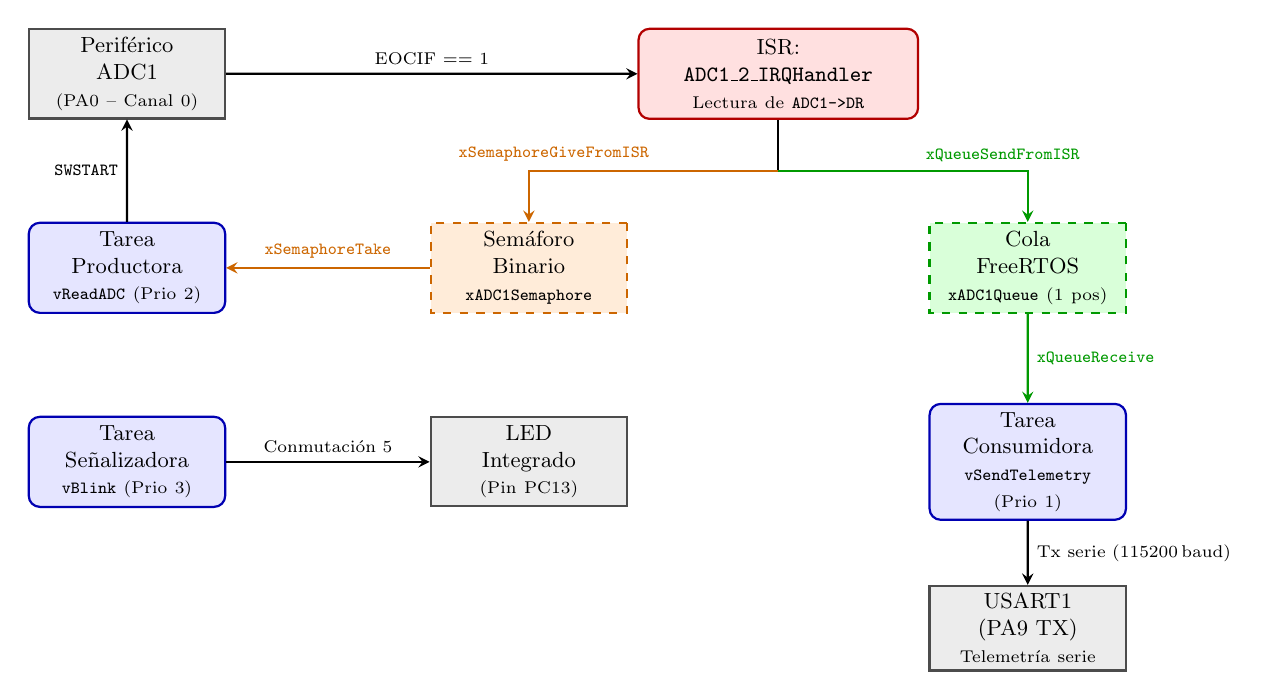
\begin{tikzpicture}[
    scale=0.88, transform shape,
    >=stealth,
    font=\small,
    block/.style={rectangle, draw=blue!70!black, thick, fill=blue!10, align=center, rounded corners=4pt, minimum height=1.3cm, text width=2.6cm},
    hw/.style={rectangle, draw=black!70, thick, fill=gray!15, align=center, minimum height=1.2cm, text width=2.6cm},
    isr/.style={rectangle, draw=red!70!black, thick, fill=red!12, align=center, rounded corners=4pt, minimum height=1.3cm, text width=3.8cm},
    queue/.style={rectangle, draw=green!60!black, thick, fill=green!15, dashed, align=center, minimum height=1.3cm, text width=2.6cm},
    sem/.style={rectangle, draw=orange!80!black, thick, fill=orange!15, dashed, align=center, minimum height=1.3cm, text width=2.6cm}
  ]

  % Fila 1: Periférico ADC e ISR (y = 4.2)
  \node[hw] (adc) at (0, 4.2) {Periférico\\ADC1\\{\scriptsize (PA0 -- Canal 0)}};
  \node[isr] (isr) at (9.4, 4.2) {ISR:\\\texttt{ADC1\_2\_IRQHandler}\\{\scriptsize Lectura de \texttt{ADC1->DR}}};

  % Fila 2: Tarea Productora y primitivas IPC (y = 1.4)
  \node[block] (task_prod) at (0, 1.4) {Tarea\\Productora\\{\scriptsize \texttt{vReadADC} (Prio 2)}};
  \node[sem] (sem) at (5.8, 1.4) {Semáforo\\Binario\\{\scriptsize \texttt{xADC1Semaphore}}};
  \node[queue] (queue) at (13.0, 1.4) {Cola\\FreeRTOS\\{\scriptsize \texttt{xADC1Queue} ($1$ pos)}};

  % Fila 3: Tarea Señalizadora, LED y Tarea Consumidora (y = -1.4)
  \node[block] (task_blink) at (0, -1.4) {Tarea\\Señalizadora\\{\scriptsize \texttt{vBlink} (Prio 3)}};
  \node[hw] (led) at (5.8, -1.4) {LED\\Integrado\\{\scriptsize (Pin PC13)}};
  \node[block] (task_cons) at (13.0, -1.4) {Tarea\\Consumidora\\{\scriptsize \texttt{vSendTelemetry} (Prio 1)}};

  % Fila 4: Periférico UART (y = -3.8)
  \node[hw] (uart) at (13.0, -3.8) {USART1\\(PA9 TX)\\{\scriptsize Telemetría serie}};

  % Punto de bifurcación desde la ISR
  \coordinate (fork) at (9.4, 2.8);

  % Conexión Productor -> ADC -> ISR
  \draw[->, thick] (task_prod) -- node[left, font=\scriptsize] {\texttt{SWSTART}} (adc);
  \draw[->, thick] (adc) -- node[above, font=\scriptsize] {EOCIF == 1} (isr);

  % Conexiones desde ISR hacia Semáforo y Cola
  \draw[thick] (isr.south) -- (fork);
  \draw[->, thick, orange!80!black] (fork) -| node[pos=0.45, above, font=\scriptsize] {\texttt{xSemaphoreGiveFromISR}} (sem.north);
  \draw[->, thick, green!60!black] (fork) -| node[pos=0.45, above, font=\scriptsize] {\texttt{xQueueSendFromISR}} (queue.north);

  % Sincronización del Productor mediante Semáforo
  \draw[->, thick, orange!80!black] (sem) -- node[above, font=\scriptsize] {\texttt{xSemaphoreTake}} (task_prod);

  % Flujo de la Cola hacia el Consumidor y Transmisión UART
  \draw[->, thick, green!60!black] (queue) -- node[right, font=\scriptsize] {\texttt{xQueueReceive}} (task_cons);
  \draw[->, thick] (task_cons) -- node[right, font=\scriptsize] {Tx serie ($115200\,\mathrm{baud}$)} (uart);

  % Señalización independiente
  \draw[->, thick] (task_blink) -- node[above, font=\scriptsize] {Conmutación $5\Hz$} (led);

\end{tikzpicture}
